In the previous exercise, the solution for Burger's equation could model the density of cars around a traffic light that turned green on $t=0$.
Another traffic model---but for high-way traffic flow in one lane where a slip road is feeding traffic into the lane---can be modeled using the initial condition
\begin{equation}\label{eq:exc3_pinit}
\rho(x, t=0) = \eta \rho_m e^{-\left(\frac{x-L/4}{L/8}\right)^2}.
\end{equation}
where $0 < \eta \le 1$ is a constant

To investigate the solution of this model. The simulation will be run for 30 time steps (equivalent to 12 seconds); the same parameters values as in exercise 2 are used but with $\eta = 0.1$ as presented in \ref{fig:exc3_congestion_eta01}, here the traffic flows rather smoothly.
If we instead increase $\eta$ to 0.9, adding higher density of traffic as presented in 
\ref{fig:exc3_congestion_eta09} we instead get congestion, increasing the density of traffic at one point at the same time decreasing the velocity at that point.


\begin{figure}[h!]
\begin{subfigure}{.375\textwidth}
	\centering
	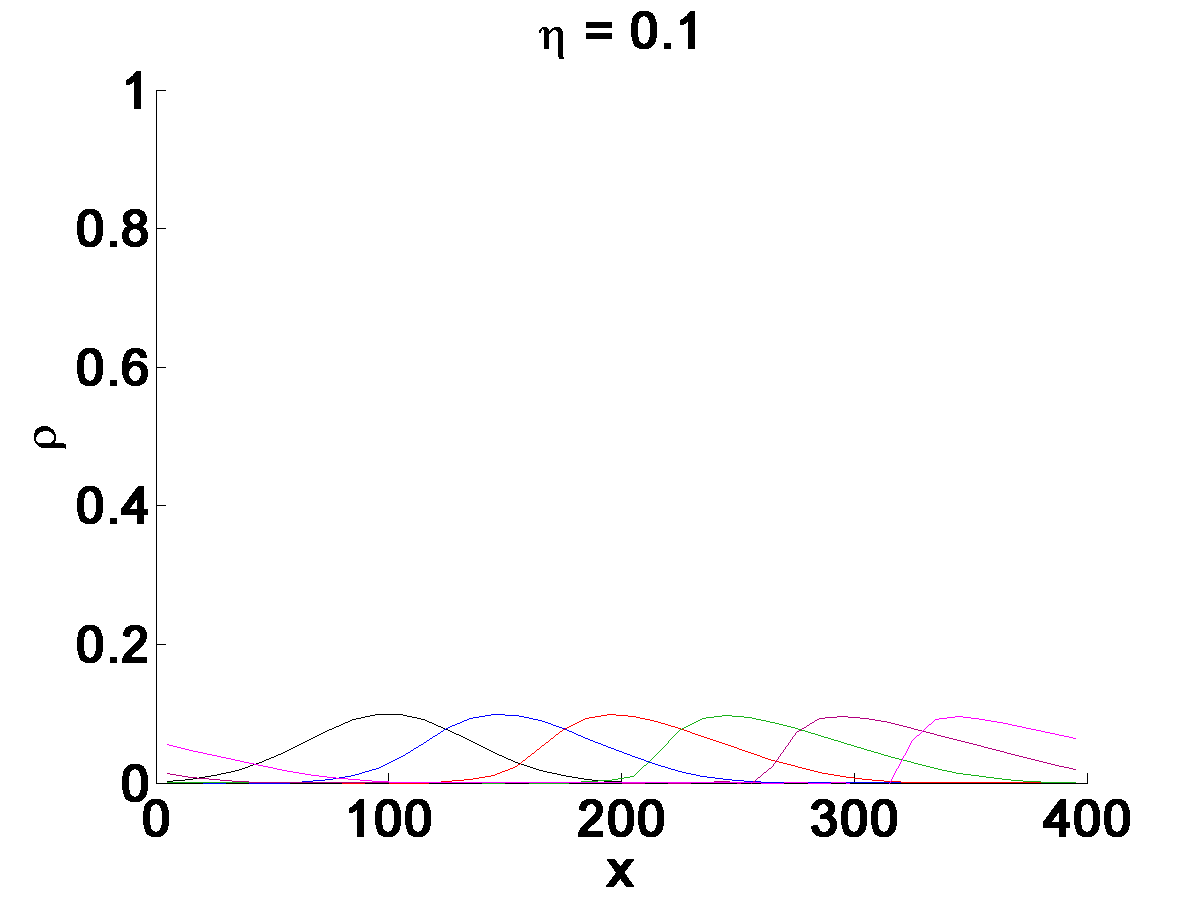
\includegraphics[width=\textwidth]{img/exc3_p_01}
	\caption{}
	\label{fig:exc3_congestion_eta01_p}
\end{subfigure}
\begin{subfigure}{.375\textwidth}
	\centering
	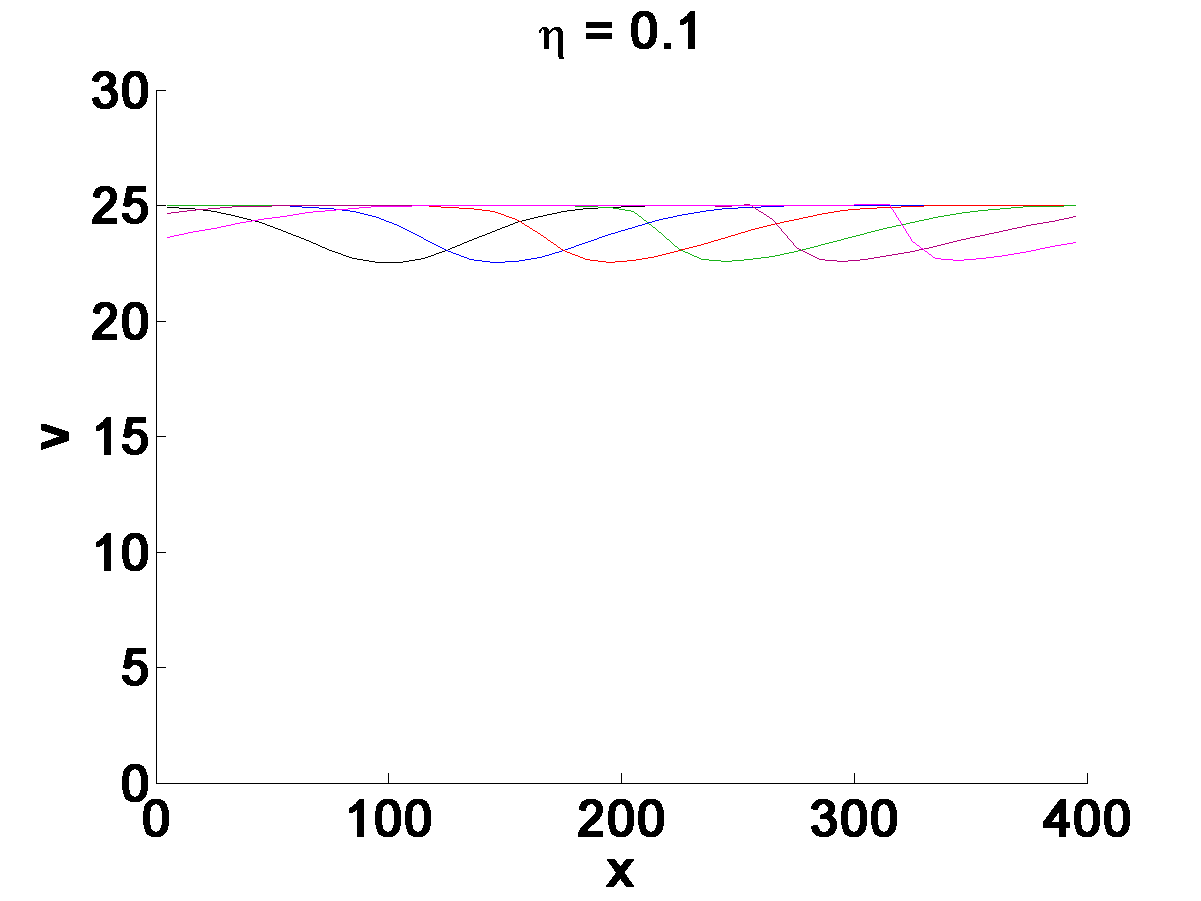
\includegraphics[width=\textwidth]{img/exc3_v_01}
	\caption{}
	\label{fig:exc3_congestion_eta01_v}
\end{subfigure}
\begin{subfigure}{.09\textwidth}
	\centering
	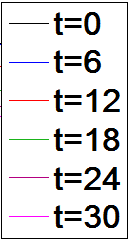
\includegraphics[width=\textwidth]{img/exc3_legend}
\end{subfigure}
\caption{The result of Burger's equation using initial condition $\rho(x, t=0) = \eta \rho_m \exp(-\left((x-L/4)/(L/8)\right)^2)$ with $\eta=0.1$. In (a) is $\rho(x)$ for different times $t$ and in (b) is $v(\rho(x))$ for different times $t$.}
\label{fig:exc3_congestion_eta01}
\end{figure}
\FloatBarrier

\begin{figure}[h!]
\begin{subfigure}{.375\textwidth}
	\centering
	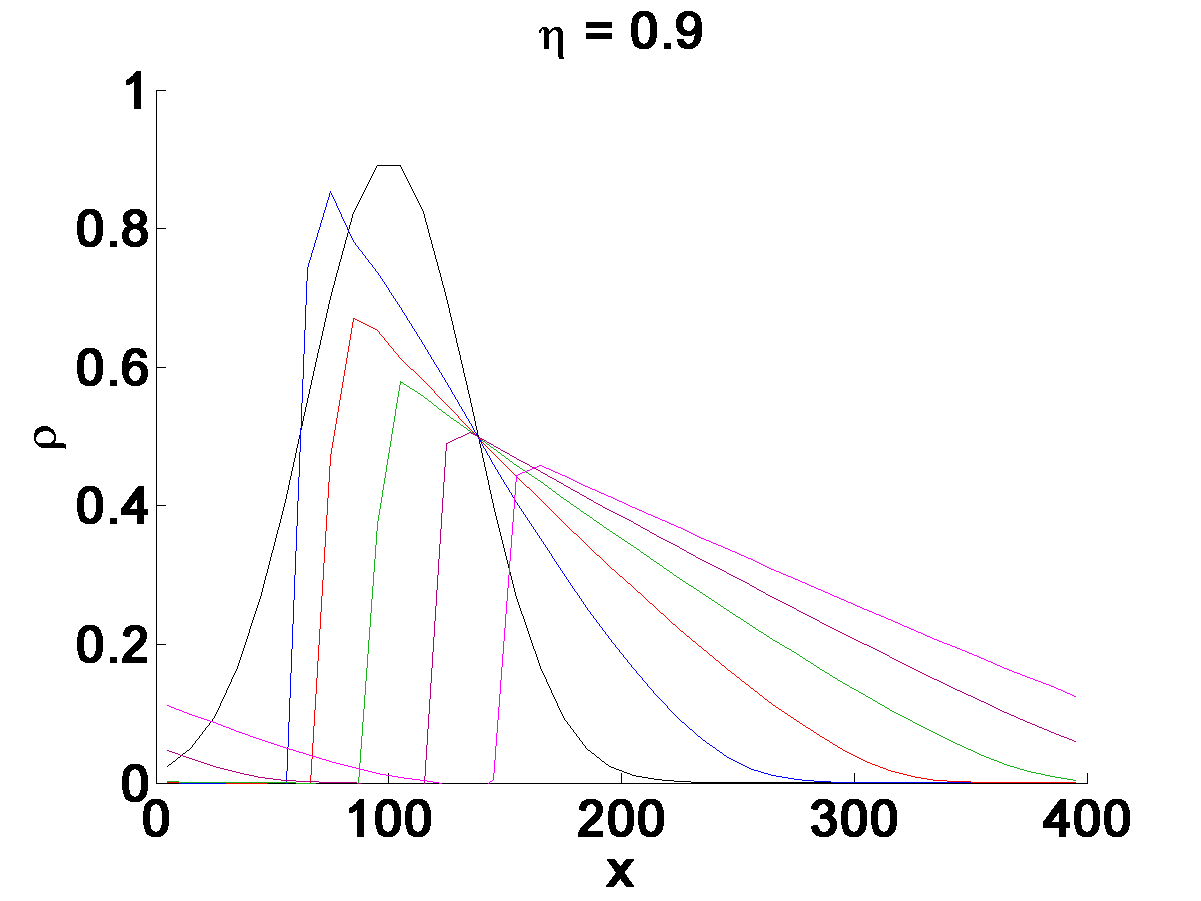
\includegraphics[width=\textwidth]{img/exc3_p_09}
	\caption{}
	\label{fig:exc3_congestion_eta01_p}
\end{subfigure}
\begin{subfigure}{.375\textwidth}
	\centering
	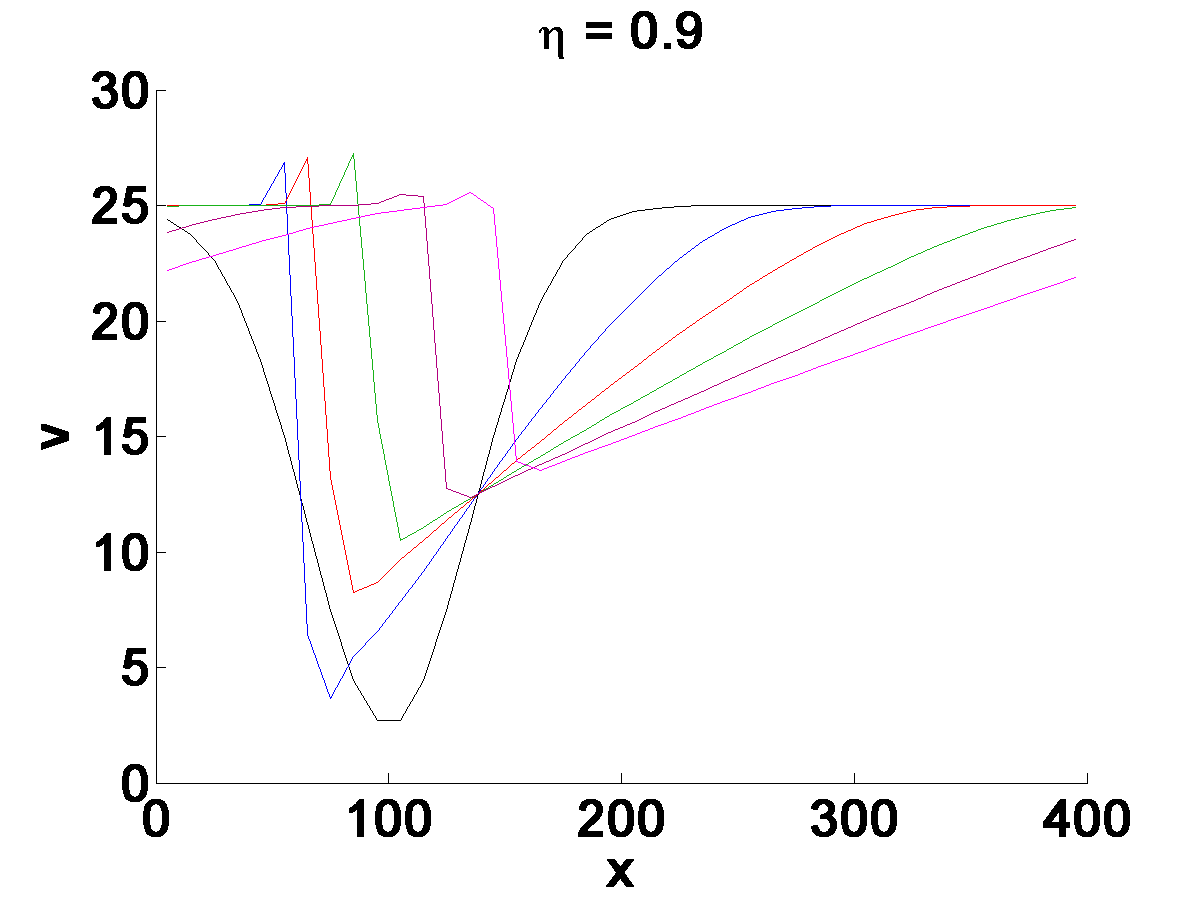
\includegraphics[width=\textwidth]{img/exc3_v_09}
	\caption{}
	\label{fig:exc3_congestion_eta01_v}
\end{subfigure}
\begin{subfigure}{.09\textwidth}
	\centering
	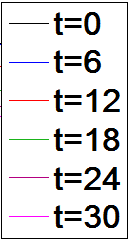
\includegraphics[width=\textwidth]{img/exc3_legend}
\end{subfigure}
\caption{The result of Burger's equation using initial condition $\rho(x, t=0) = \eta \rho_m \exp(-\left((x-L/4)/(L/8)\right)^2)$ with $\eta=0.9$. In (a) is $\rho(x)$ for different times $t$ and in (b) is $v(\rho(x))$ for different times $t$.}
\label{fig:exc3_congestion_eta09}
\end{figure}
\FloatBarrier